\apendice{Documentación de usuario}

\section{Introducción}
En este apéndice se explican los requisitos que debe cumplir el usuario para ejecutar la aplicación, cómo lanzarla y cómo usarla.

\section{Requisitos de usuarios}
Al tratarse de una aplicación web, los requisitos que debe cumplir el usuario son los siguientes:

\begin{itemize}
	\tightlist
	\item Navegador web instalado, la aplicación se ha probado en \textit{Firefox} y \textit{Chrome}.
	\item JavaScript activo en el navegador.
\end{itemize}


\section{Instalación}
Debido a que se proporciona una aplicación web, no es necesario instalarla para poder usarla. Sin embargo, si se quiere proceder a la instalación, se pueden seguir las instrucciones en la sección \ref{sec:instalacion}.


\section{Manual del usuario}
En esta sección se enseña al usuario como manejar la aplicación.

\subsection{Inicio}
Nada más entrar a la aplicación, se muestra la pantalla de inicio (figura~\ref{fig:inicio}). En ella se puede ver un texto de presentación de la aplicación web y se da acceso al resto de funcionalidades.

\begin{figure}[h]
	\centering
	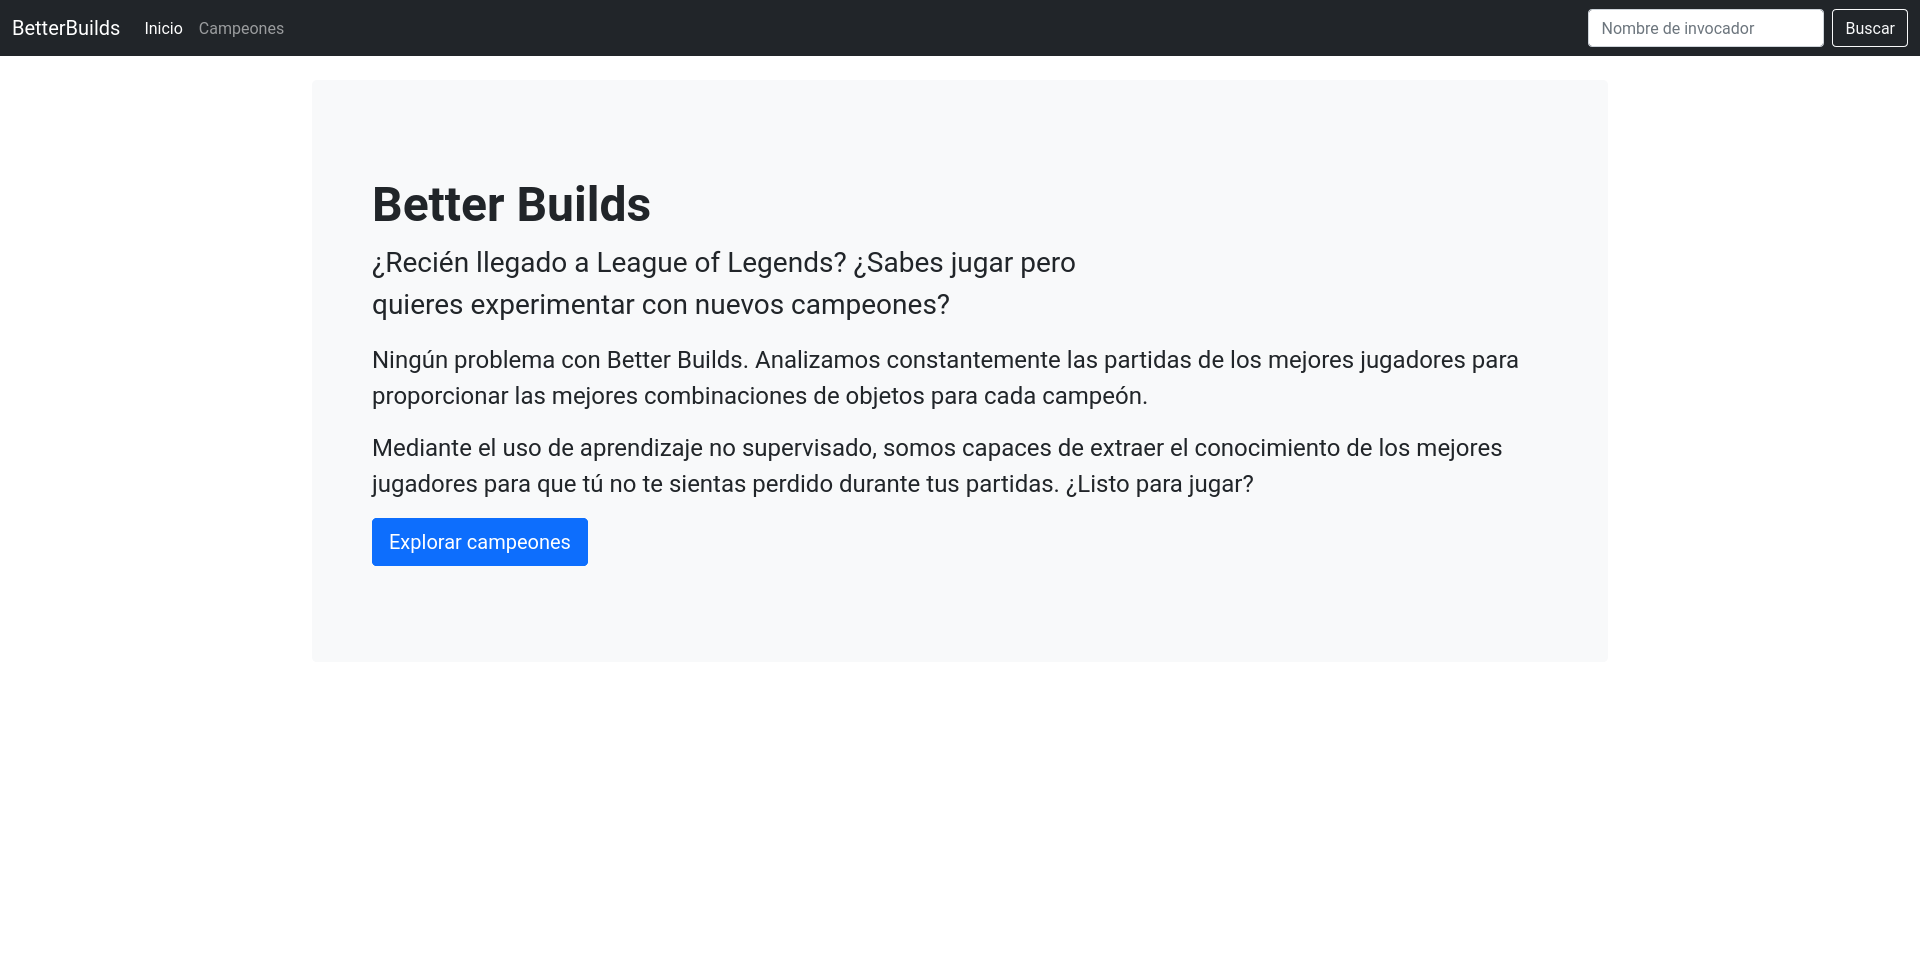
\includegraphics[width=1\linewidth]{img/0.inicio}
	\caption{Pantalla de inicio}
	\label{fig:inicio}
\end{figure}

Desde aquí se puede navegar al listado de campeones (sección~\ref{sec:listado}) y se puede buscar una partida en curso (sección~\ref{sec:partida}). Al estar localizados los enlaces en la cabecera, también se puede acceder desde el resto de la aplicación.

\subsection{Listado de campeones}\label{sec:listado}
En esta pantalla se presenta un listado con todos los campeones actuales del juego (figura~\ref{fig:listado}). También se encuentra un buscador con el que se puede filtrar el listado (figura~\ref{fig:buscador}), para encontrar de forma más rápida a un campeón concreto.

\begin{figure}[h]
	\centering
	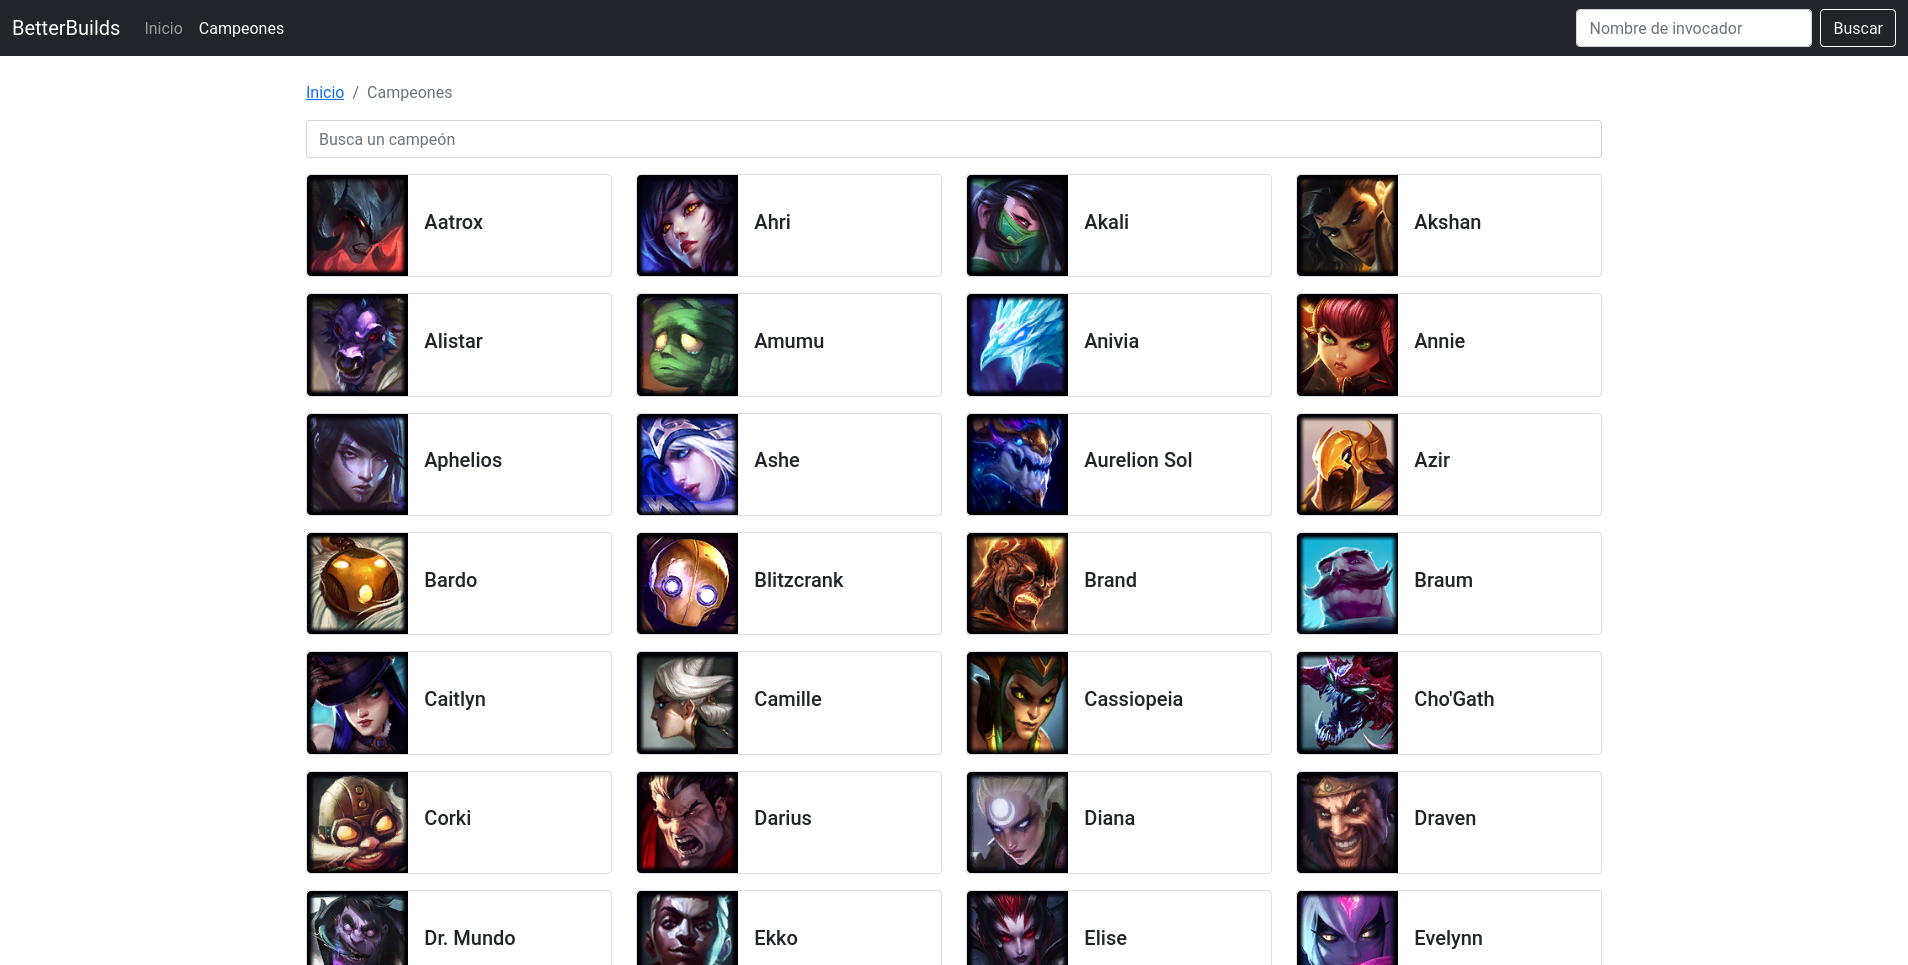
\includegraphics[width=1\linewidth]{img/1.listado}
	\caption{Listado de campeones}
	\label{fig:listado}
\end{figure}
\begin{figure}[h]
	\centering
	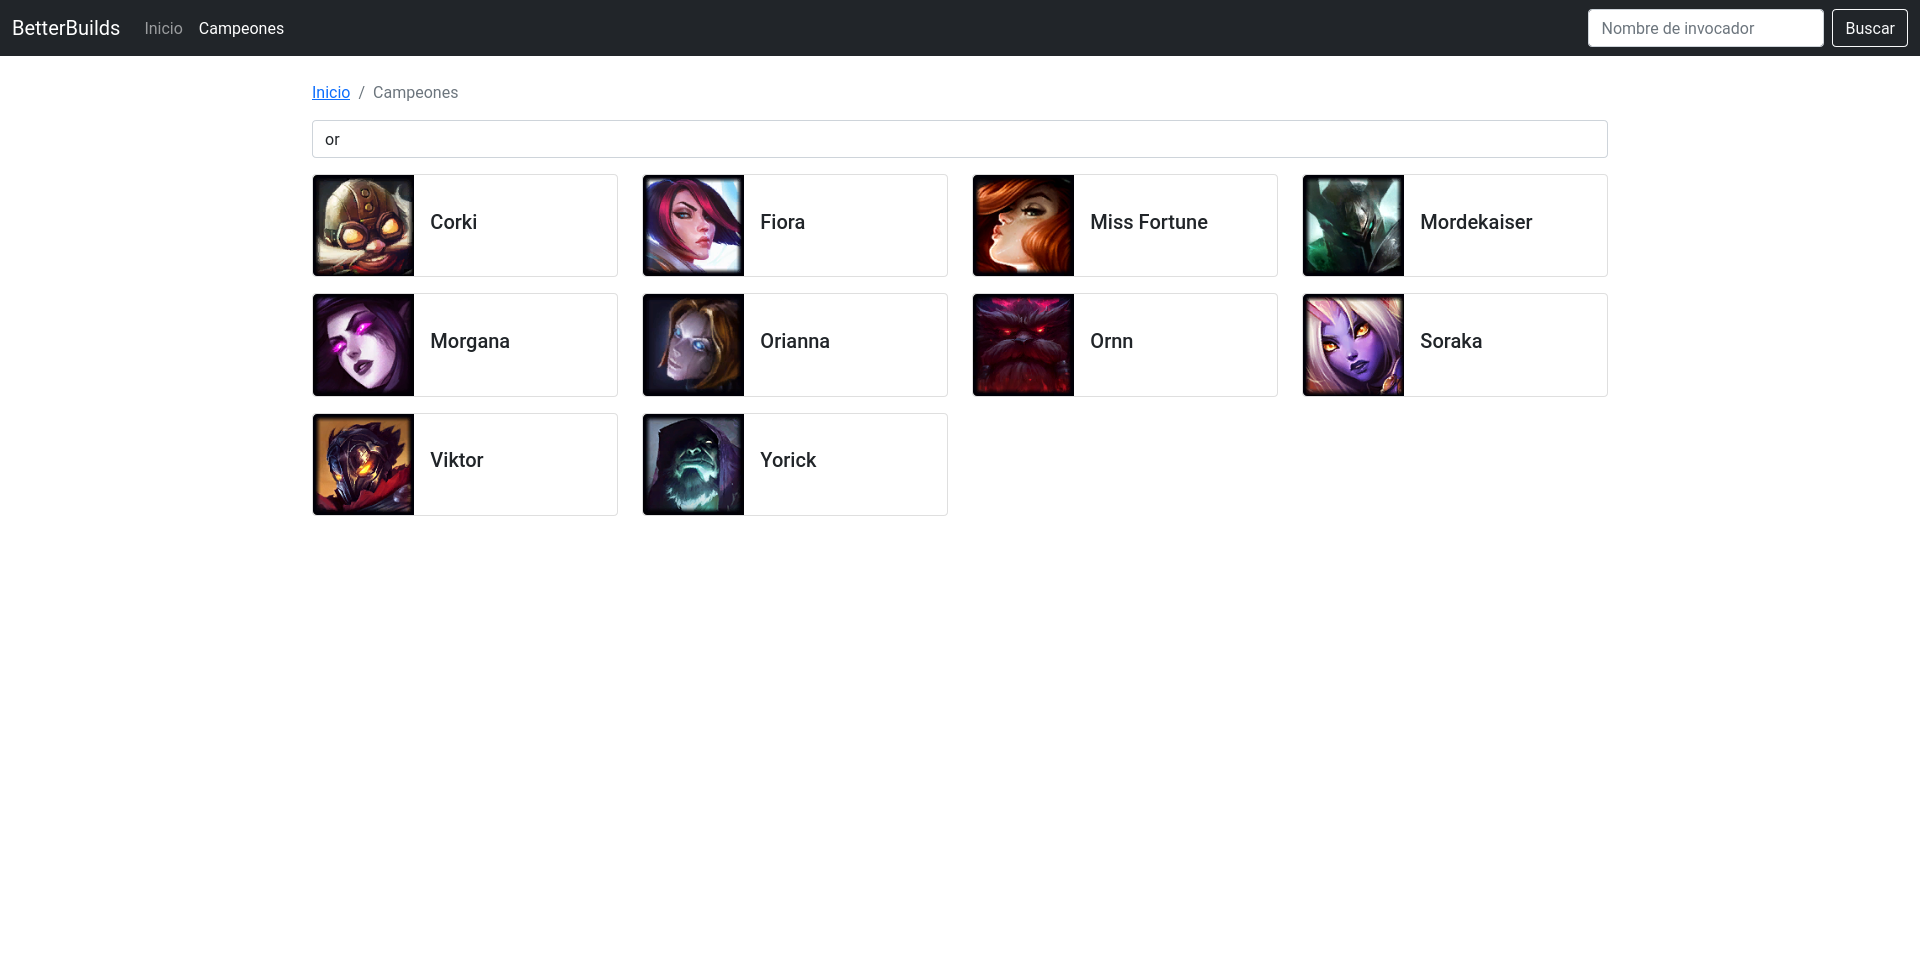
\includegraphics[width=1\linewidth]{img/2.buscador}
	\caption{Buscador}
	\label{fig:buscador}
\end{figure}

Una vez localizado el campeón se puede pinchar en él para navegar hacia su ficha (sección~\ref{sec:ficha}) y consultar los conjuntos de objetos.

\subsection{Ficha del campeón}\label{sec:ficha}
La ficha del campeón (figura~\ref{fig:ficha} y \ref{fig:ficha2}) se divide en una sección de presentación y en otra con los conjuntos de objetos. En la parte de presentación se muestra la foto del campeón, el número de partidas analizadas, un texto sobre la historia del mismo y consejos para su manejo en partida.

\begin{figure}[h]
	\centering
	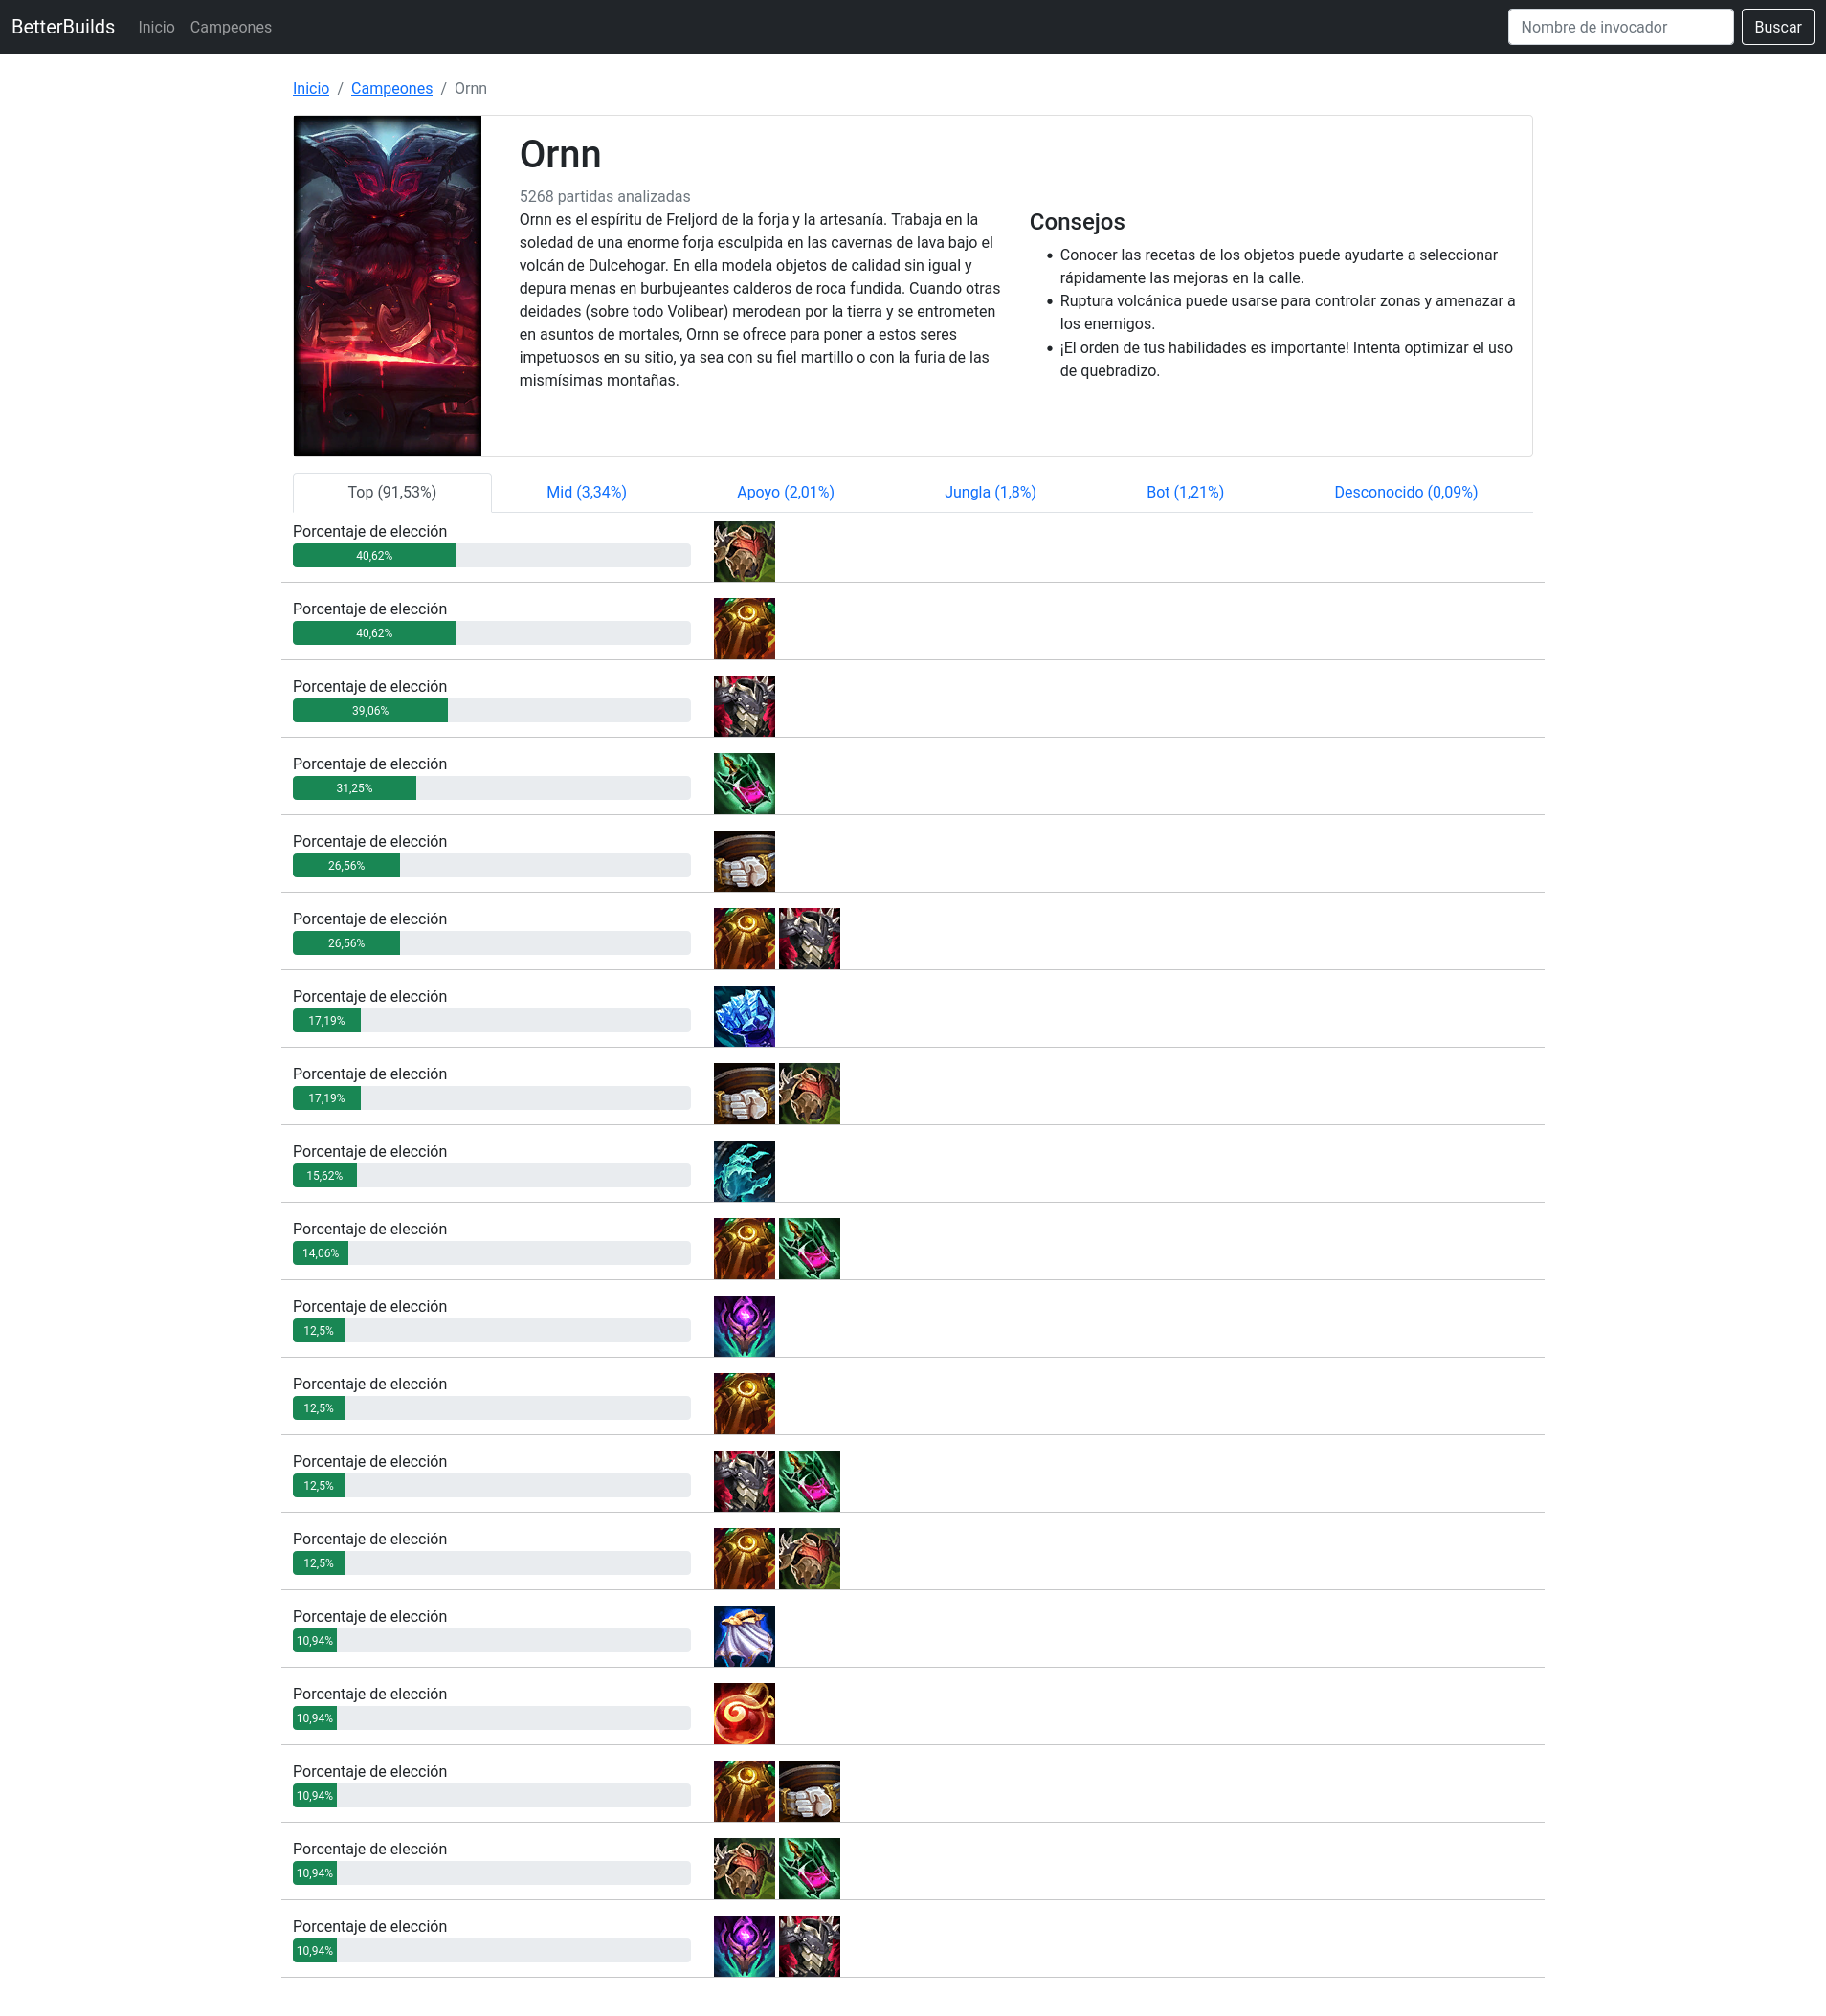
\includegraphics[width=1\linewidth]{img/3.campeon}
	\caption{Ficha del campeón}
	\label{fig:ficha}
\end{figure}
\begin{figure}[h]
	\centering
	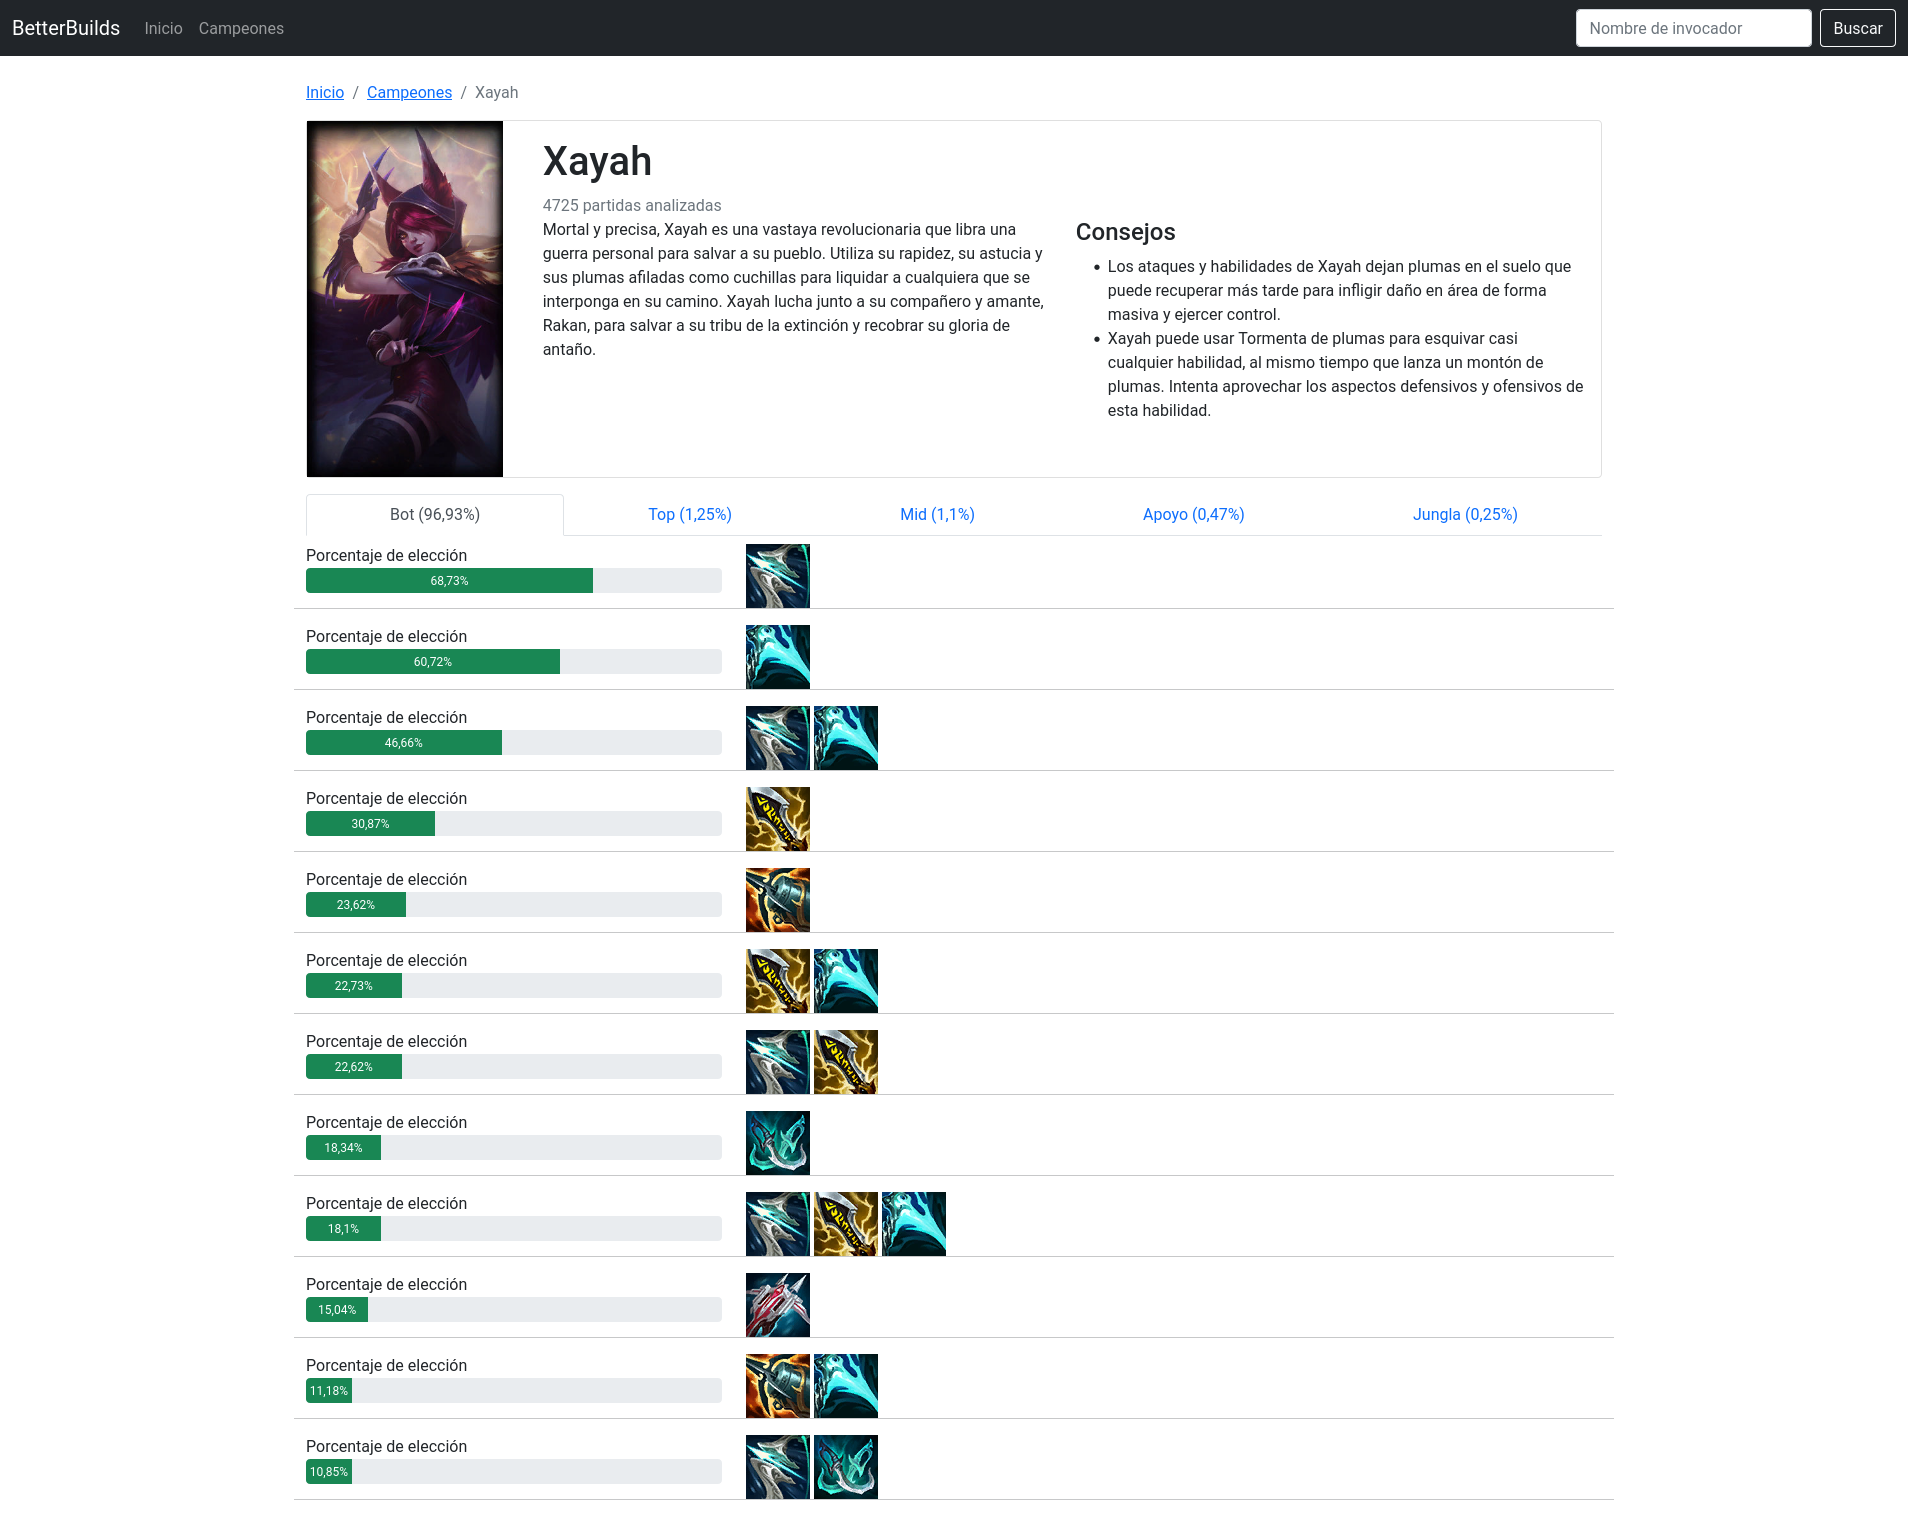
\includegraphics[width=1\linewidth]{img/4.campeon}
	\caption{Ficha de otro campeón}
	\label{fig:ficha2}
\end{figure}

La parte de los objetos está dividida en pestañas, una para cada posición y una extra para las partidas en las que no ha sido posible identificarla. Se encuentran ordenadas por el porcentaje de partidas jugadas en esa posición.

Dentro de cada pestaña la estructura es similar. Se presenta un listado con los conjuntos de objetos que se han obtenido del análisis de partidas, junto con el porcentaje de elección de esa combinación, representado por una barra de progreso, para una mejor usabilidad. Los conjuntos se encuentran ordenados por este porcentaje.

\subsection{Partida actual}\label{sec:partida}
Para los jugadores que estén en partida y quieran realizar una consulta sobre el campeón que están jugando actualmente, se da la opción de poder buscarse a sí mismos mediante el apodo dentro del juego. Esta búsqueda lleva directamente al jugador a la ficha del personaje con el que se encuentra jugando (figura~\ref{fig:partida}).

\begin{figure}[h]
	\centering
	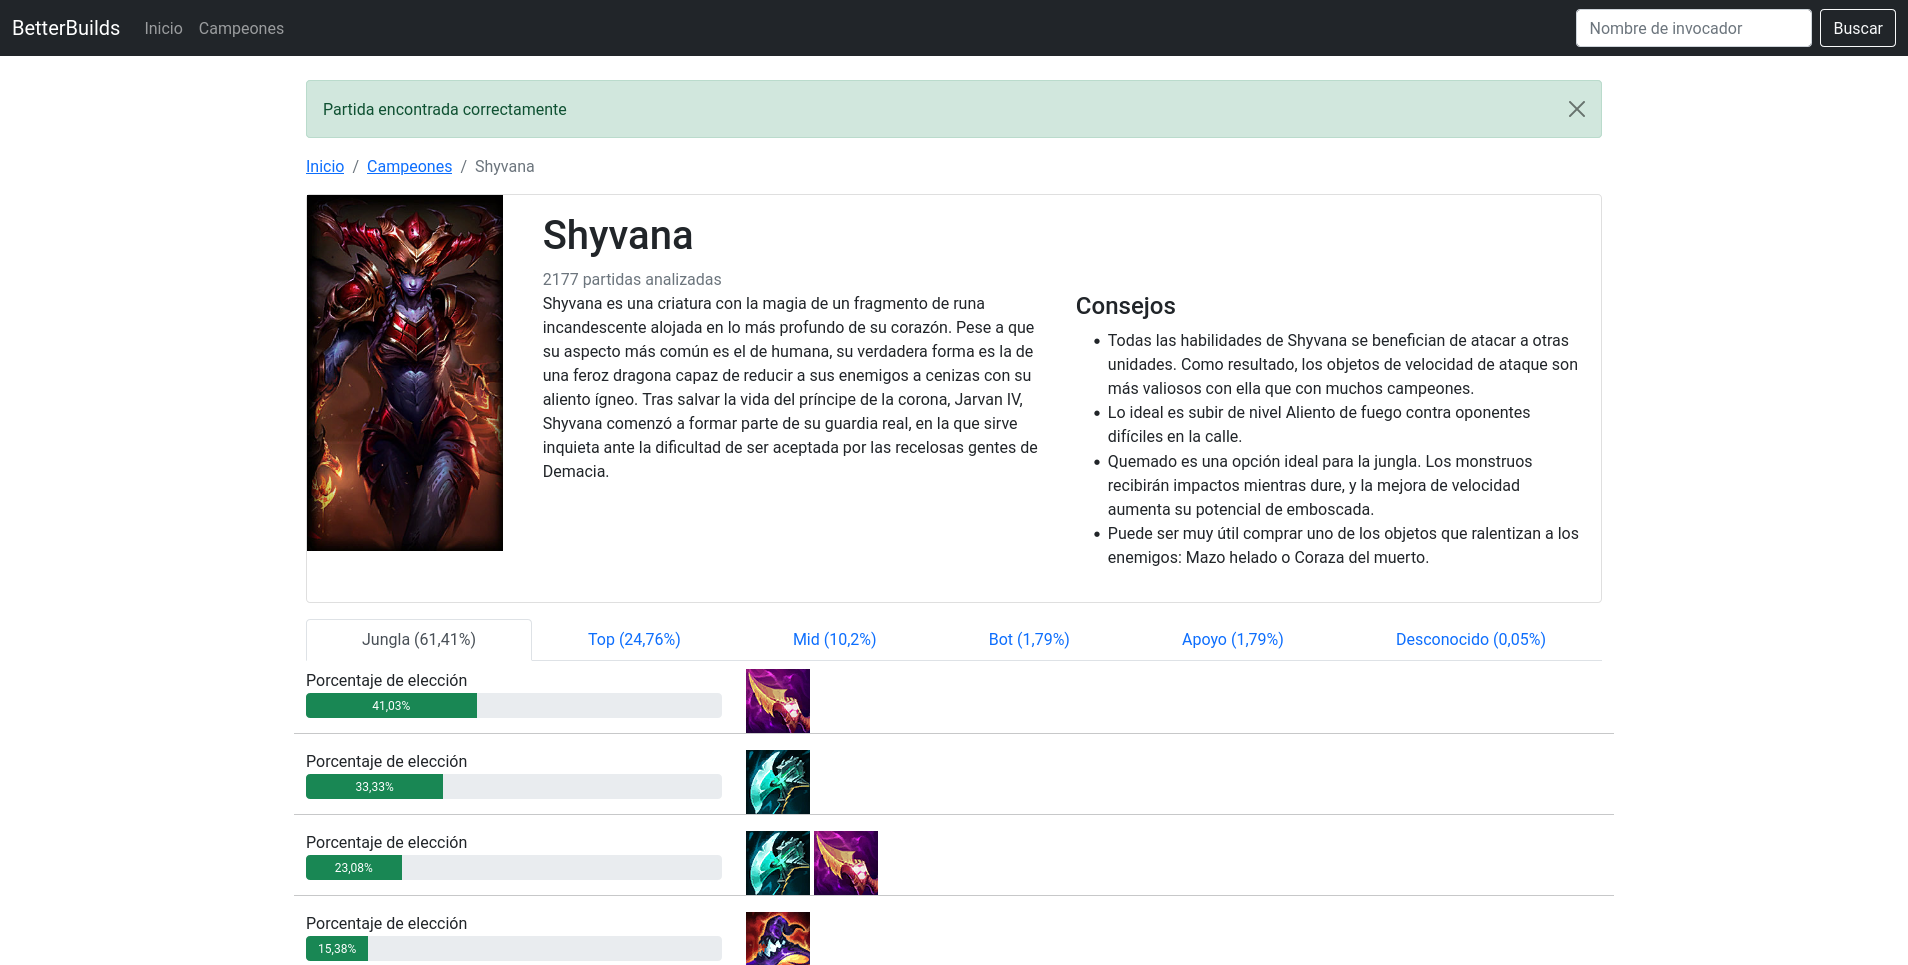
\includegraphics[width=1\linewidth]{img/5.partida}
	\caption{Búsqueda por jugador}
	\label{fig:partida}
\end{figure}

En el caso de que el jugador no se encuentre en partida para el jugador buscado (figura~\ref{fig:no-partida}) o no exista el jugador (figura~\ref{fig:no-existes}), se muestra un mensaje de error avisando al usuario.

\begin{figure}[h]
	\centering
	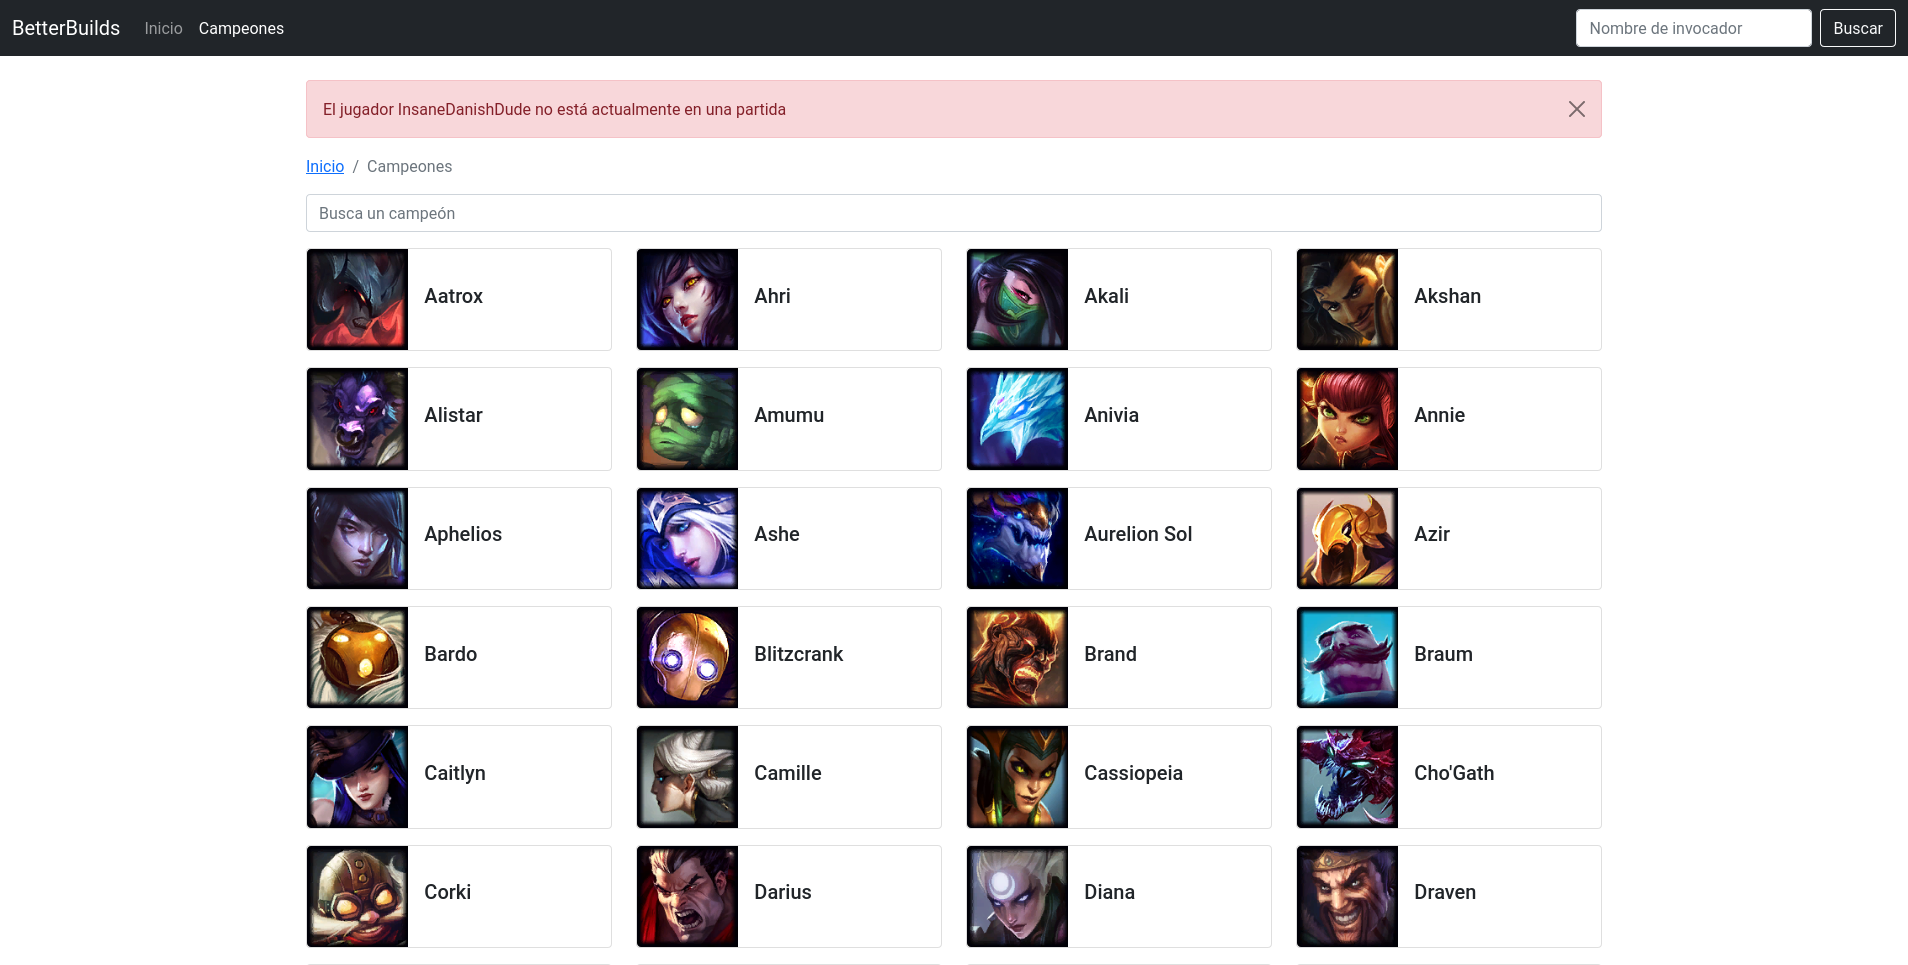
\includegraphics[width=1\linewidth]{img/6.no-partida}
	\caption{El jugador no está en partida}
	\label{fig:no-partida}
\end{figure}
\begin{figure}
	\centering
	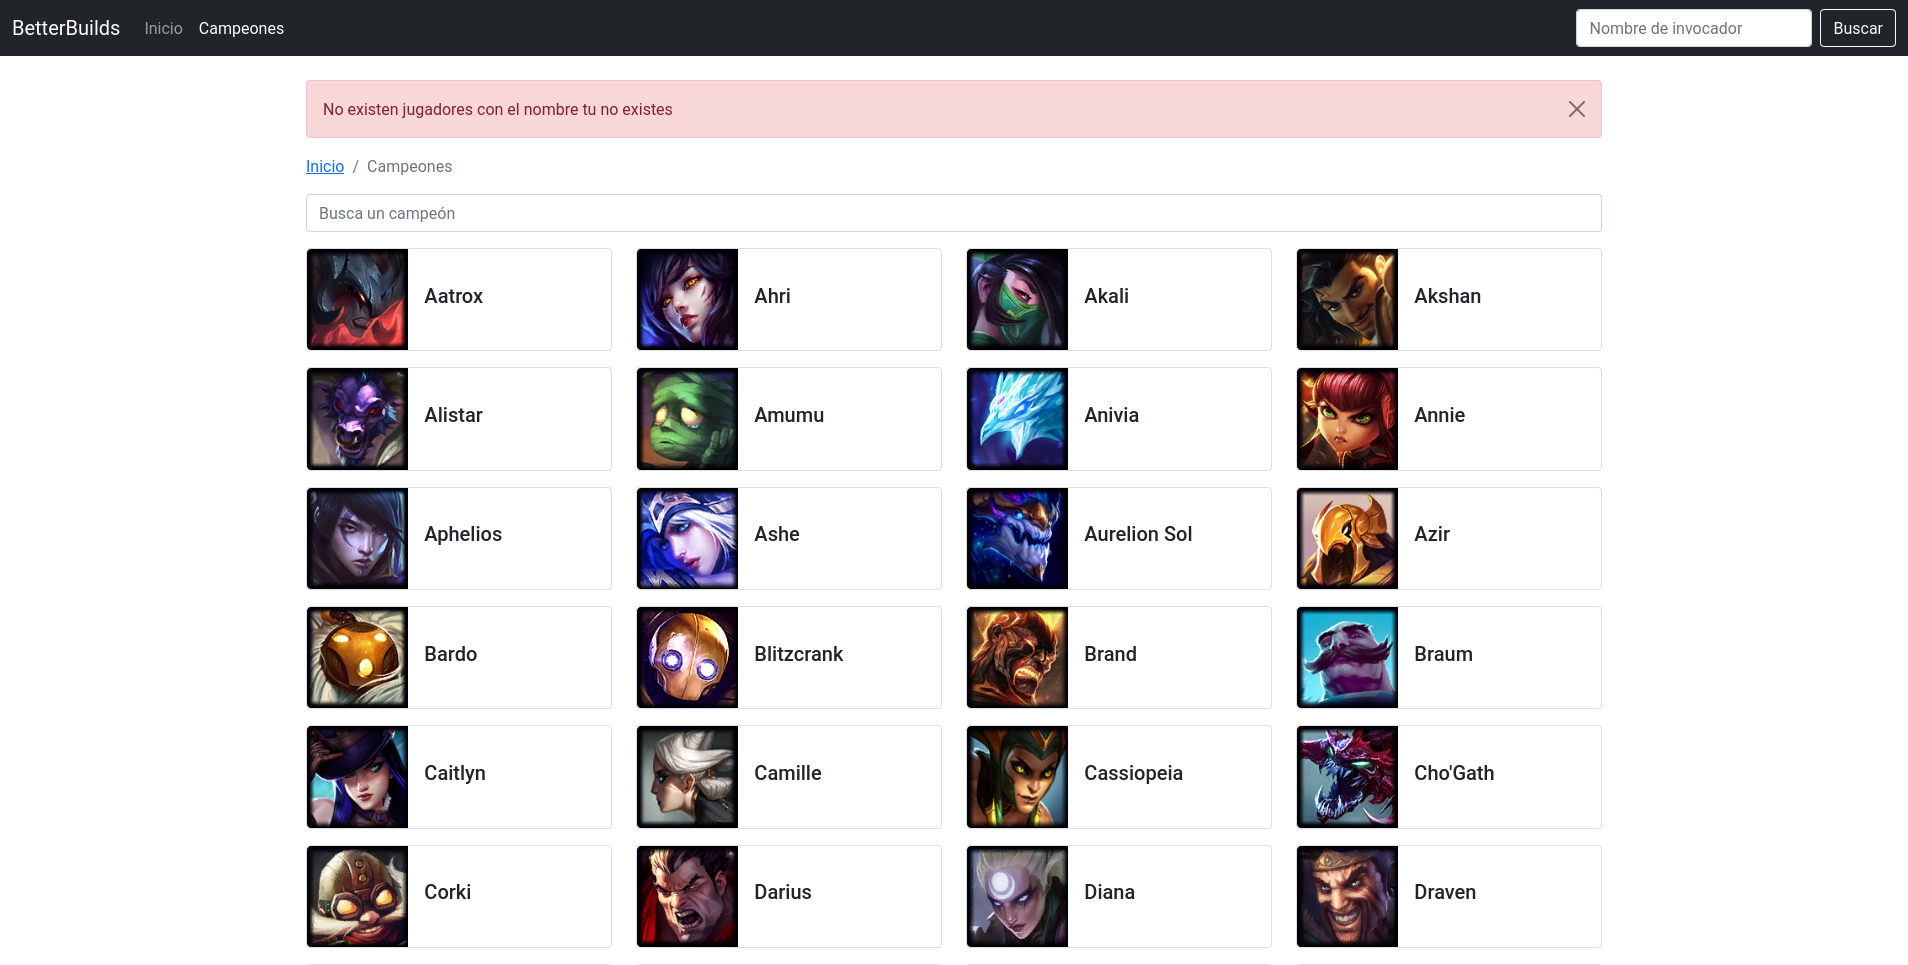
\includegraphics[width=1\linewidth]{img/7.no-existes}
	\caption{No existe el jugador con el nombre introducido}
	\label{fig:no-existes}
\end{figure}
